\subsection{Model Optimizations} \label{subsec:mdopti}
As mentioned previously, the major issues, when implementing an \acrshort{cnn} on a \acrshort{fpga}, are the \acrshort{cnn} size and its computational complexity. The research was made to develop techniques to tackle those two issues by directly modifying the \acrshort{cnn} architecture. \textcite{nurvitadhi_can_2017} believe that sparsity exploitation and extremely compact data types will become the norm in next-generation \acrshort{cnn}s.
%
%
\subsubsection{Efficient Model Design}
%
Section \ref{subsec:models} presented several state of the art models. However, those models (except MobileNetV2) were designed to provide the highest performance possible but did not consider the implementation of such models on mobile and embedded devices \cite{iandola_squeezenet_2016}. Therefore, several other models were designed to run on such constrained platforms trading a reduction of the number of parameters and operations in exchange for a drop of accuracy. Indeed, if we observe Figure \ref{fig:archi}, the lightweight models do not match the high-performance ones in terms of accuracy only.

A clever choice of design decreases the number of parameters and computations of the model while reducing the drop of accuracy. As many approaches were proposed to reduce the size of a model, this study will focus on architectures that target the embedded space. This section describes five of these architectures:
\begin{itemize}
    \item \textbf{SqueezeNet} \cite{iandola_squeezenet_2016} was focused on reducing the number of parameters of AlexNet (see Section \ref{subsec:models}) by introducing a new building block: \textbf{Fire Module}. Therefore, their architectures are very similar. SqueezeNet replaces all layers (except the first and last one) by \textbf{Fire Modules}. The \textbf{Fire Module}, observed in Figure \ref{fig:archi_building_block:sqn}, is composed of two convolutional layers. The first one called \textit{squeeze block} only performs $1 \times 1$ convolutions to squeeze the number of input channels. The reduction of the number of channels decreases the computational complexity and number of parameters of the next convolutional layer. Moreover, they also chose $1 \times 1$ convolution because it requires fewer parameters than $3 \times 3$ convolution.
    The second convolutional layer called \textit{expand block} is composed of $1 \times 1$ and $3 \times 3$ convolutions. With this architecture, the size of AlexNet is decreased from $240$MB to $4.8$MB \cite{iandola_squeezenet_2016}. It can even be reduced to $0.47$MB without a drop in accuracy method by applying Deep Compression \cite{han_deep_2016}. However, it has a big memory footprint, is slower in runtime, and consumes more energy than AlexNet \cite{sze_efficient_2017}.
    %
    \item \textbf{MobileNet} \cite{howard_mobilenets_2017} uses \acrshort{dsc}, described in Section \ref{subs:dsc}, to build small and low latency models that can fulfill the design requirements, as can be seen in Figure \ref{fig:archi_building_block:mbn}. Two hyper-parameters are used to set the model size and throughput:
    %
    \begin{itemize}
        \item The width multiplier $\alpha \in [1; 0[$, which reduces the number of input and output channel at each layer,
        \item The resolution multiplier $\rho \in [1; 0[$,  which reduces spatially the input and output \acrshort{fm} at each layer.
    \end{itemize}
    %
    \item \textbf{ShuffleNet}  was developed by \textcite{zhang_shufflenet_2018}, in 2018. It is designed to be a computation-efficient architecture, especially for mobile devices with very limited computing power. Indeed, it reduces the computation cost while maintaining the accuracy by using \textbf{pointwise group convolution}, decreasing the computation complexity of $1 \times 1$ convolutions. It also uses \textbf{channel shuffle} operation on the channels such that \textbf{group convolutions} obtain information from different groups. Then more powerful structures can be built with multiple group convolutional layers. However, the group convolutions and the bottleneck structures add \acrfull{mac} which is a non-negligible cost \cite{ma_shufflenet_2018}. The group convolution contributes to network fragmentation and reduces parallelism. Moreover, the \textquote{Add} operation, as seen in Figure \ref{fig:archi_building_block:shn}, is non-negligible too.
    %,
    \item \textbf{NasNet} was developed by \textcite{zoph_learning_2018}, in 2018. The idea was to use a search method called \acrfull{nas}, to find good convolutional architectures on a specific dataset. For that purpose, NasNet uses a \acrfull{rnn} to generate efficient architectures. The \acrshort{rnn} generates sample child networks with different architectures, which are trained to convergence. The accuracy of the child networks is used to train the \acrshort{rnn}, which will generate better architectures over time. A convolution layer can be seen in Figure \ref{fig:archi_building_block:nasn}. The learned architecture is flexible as it may be scaled in terms of computational cost. The network provides a higher accuracy with comparable parameters and \acrshort{mac} than MobileNet and ShuffleNet (described previously) \cite{zoph_learning_2018}. However, the resulting network ends up very complex \cite{sandler_mobilenetv2_2018}.
    %
    \item \textbf{MobileNetV2} was developed by \textcite{sandler_mobilenetv2_2018}, in 2018. It is an improvement of MobileNet (described previously) in terms of accuracy and does not require special operators. It has also a smaller memory footprint. Furthermore, MobileNetV2 has a faster inference and fewer parameters to MobileNet. MobileNetV2 has already been explained in Section \ref{subs:mbv2}.
\end{itemize}
%
\begin{figure}[H]
    \centering
    %
    \begin{subfigure}[t]{0.49\linewidth}
        \centering
        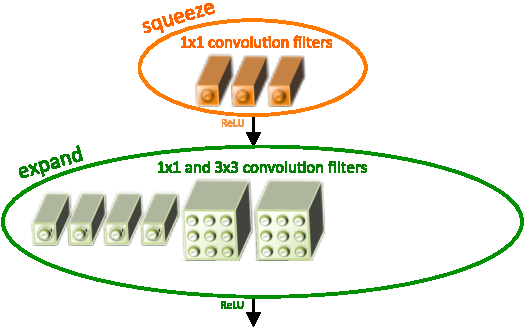
\includegraphics[width=\textwidth, height=0.3\textheight, keepaspectratio]{squeeze.pdf}
        \caption{Squeezenet Fire Module\cite{iandola_squeezenet_2016}}
        \label{fig:archi_building_block:sqn}
    \end{subfigure}
    %
    \begin{subfigure}[t]{0.49\linewidth}
        \centering
        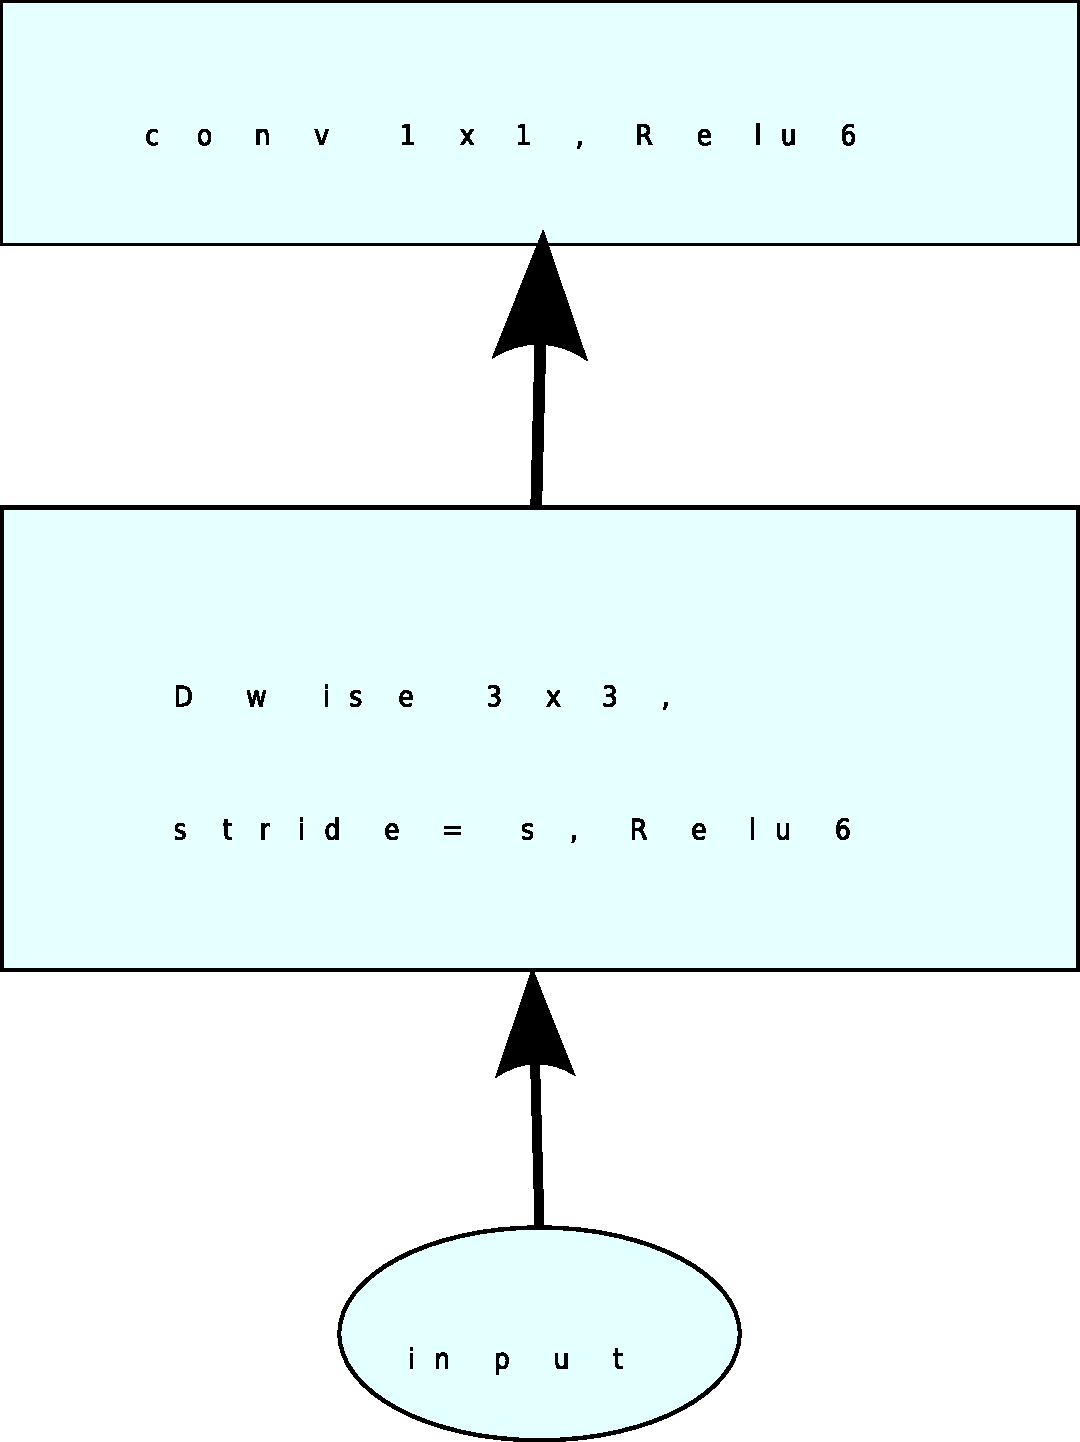
\includegraphics[width=\textwidth, height=0.2\textheight, keepaspectratio]{mobilenet.pdf}
        \caption{MobileNet convolutional block \cite{howard_mobilenets_2017}}
        \label{fig:archi_building_block:mbn}
    \end{subfigure}
    %
    \begin{subfigure}[t]{0.49\linewidth}
        \centering
        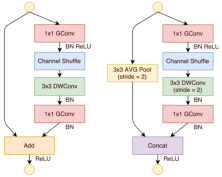
\includegraphics[width=\textwidth, height=0.2\textheight, keepaspectratio]{shufflenet.pdf}
        \caption{ShuffleNet convolutional block \cite{zhang_shufflenet_2018}}
        \label{fig:archi_building_block:shn}
    \end{subfigure}
    %
    \begin{subfigure}[t]{0.49\linewidth}
        \centering
        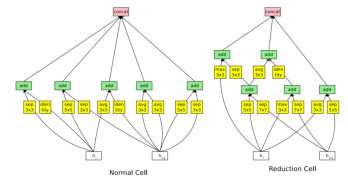
\includegraphics[width=\textwidth, height=0.3\textheight, keepaspectratio]{nasnet.pdf}
        \caption{NasNet convolutional blocks \cite{zoph_learning_2018}}
        \label{fig:archi_building_block:nasn}
    \end{subfigure}
    %
    \begin{subfigure}[t]{0.49\linewidth}
        \centering
        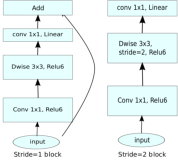
\includegraphics[width=\textwidth, height=0.2\textheight, keepaspectratio]{mobilenet2.pdf}
        \caption{MobileNetv2 convolutional blocks \cite{sandler_mobilenetv2_2018}}
        \label{fig:archi_building_block:mb2n}
    \end{subfigure}
    %
    \caption{Convolutional block from different architectures}
    \label{fig:archi_building_block}
\end{figure}

The architecture presented by this work was developed to implement MobileNetV2 because of its simplicity and its state-of-the-art performance (see Table \ref{tab:mbv2}). Moreover, MobileNetV2 requires fewer parameters while providing state-of-art accuracy when comparing to the different architectures, as shown in Figure \ref{fig:archi}.
%
\begin{table}[H]
    \center
    \begin{tabular}{ | c | c | c c | c| }
        \hline \hline
        Network & Top 1 & Params & MAdds & CPU \\
        \hline \hline
        MobileNetV1 & 70.6 & 4.2M & 575M & 113ms \\
        ShuffleNet (1.5) & 71.5 & \textbf{3.4M} & 292M & - \\
        ShuffleNet (x2)  & 73.7 & 5.4M & 524M & - \\
        NasNet-A & 74.0 & 5.3M & 564M & 183ms \\
        \hline
        MobileNetV2 & \textbf{72.0} & \textbf{3.4M} & \textbf{300M} & \textbf{75ms} \\
        MobileNetV2 (1.4) & \textbf{74.7} & 6.9M & 585M & \textbf{143ms} \\
        \hline \hline
    \end{tabular}
    \caption{Performance on ImageNet, comparison for different networks \cite{sandler_mobilenetv2_2018}}
    \label{tab:mbv2}
\end{table}

\begin{figure}[H]
    \centering
    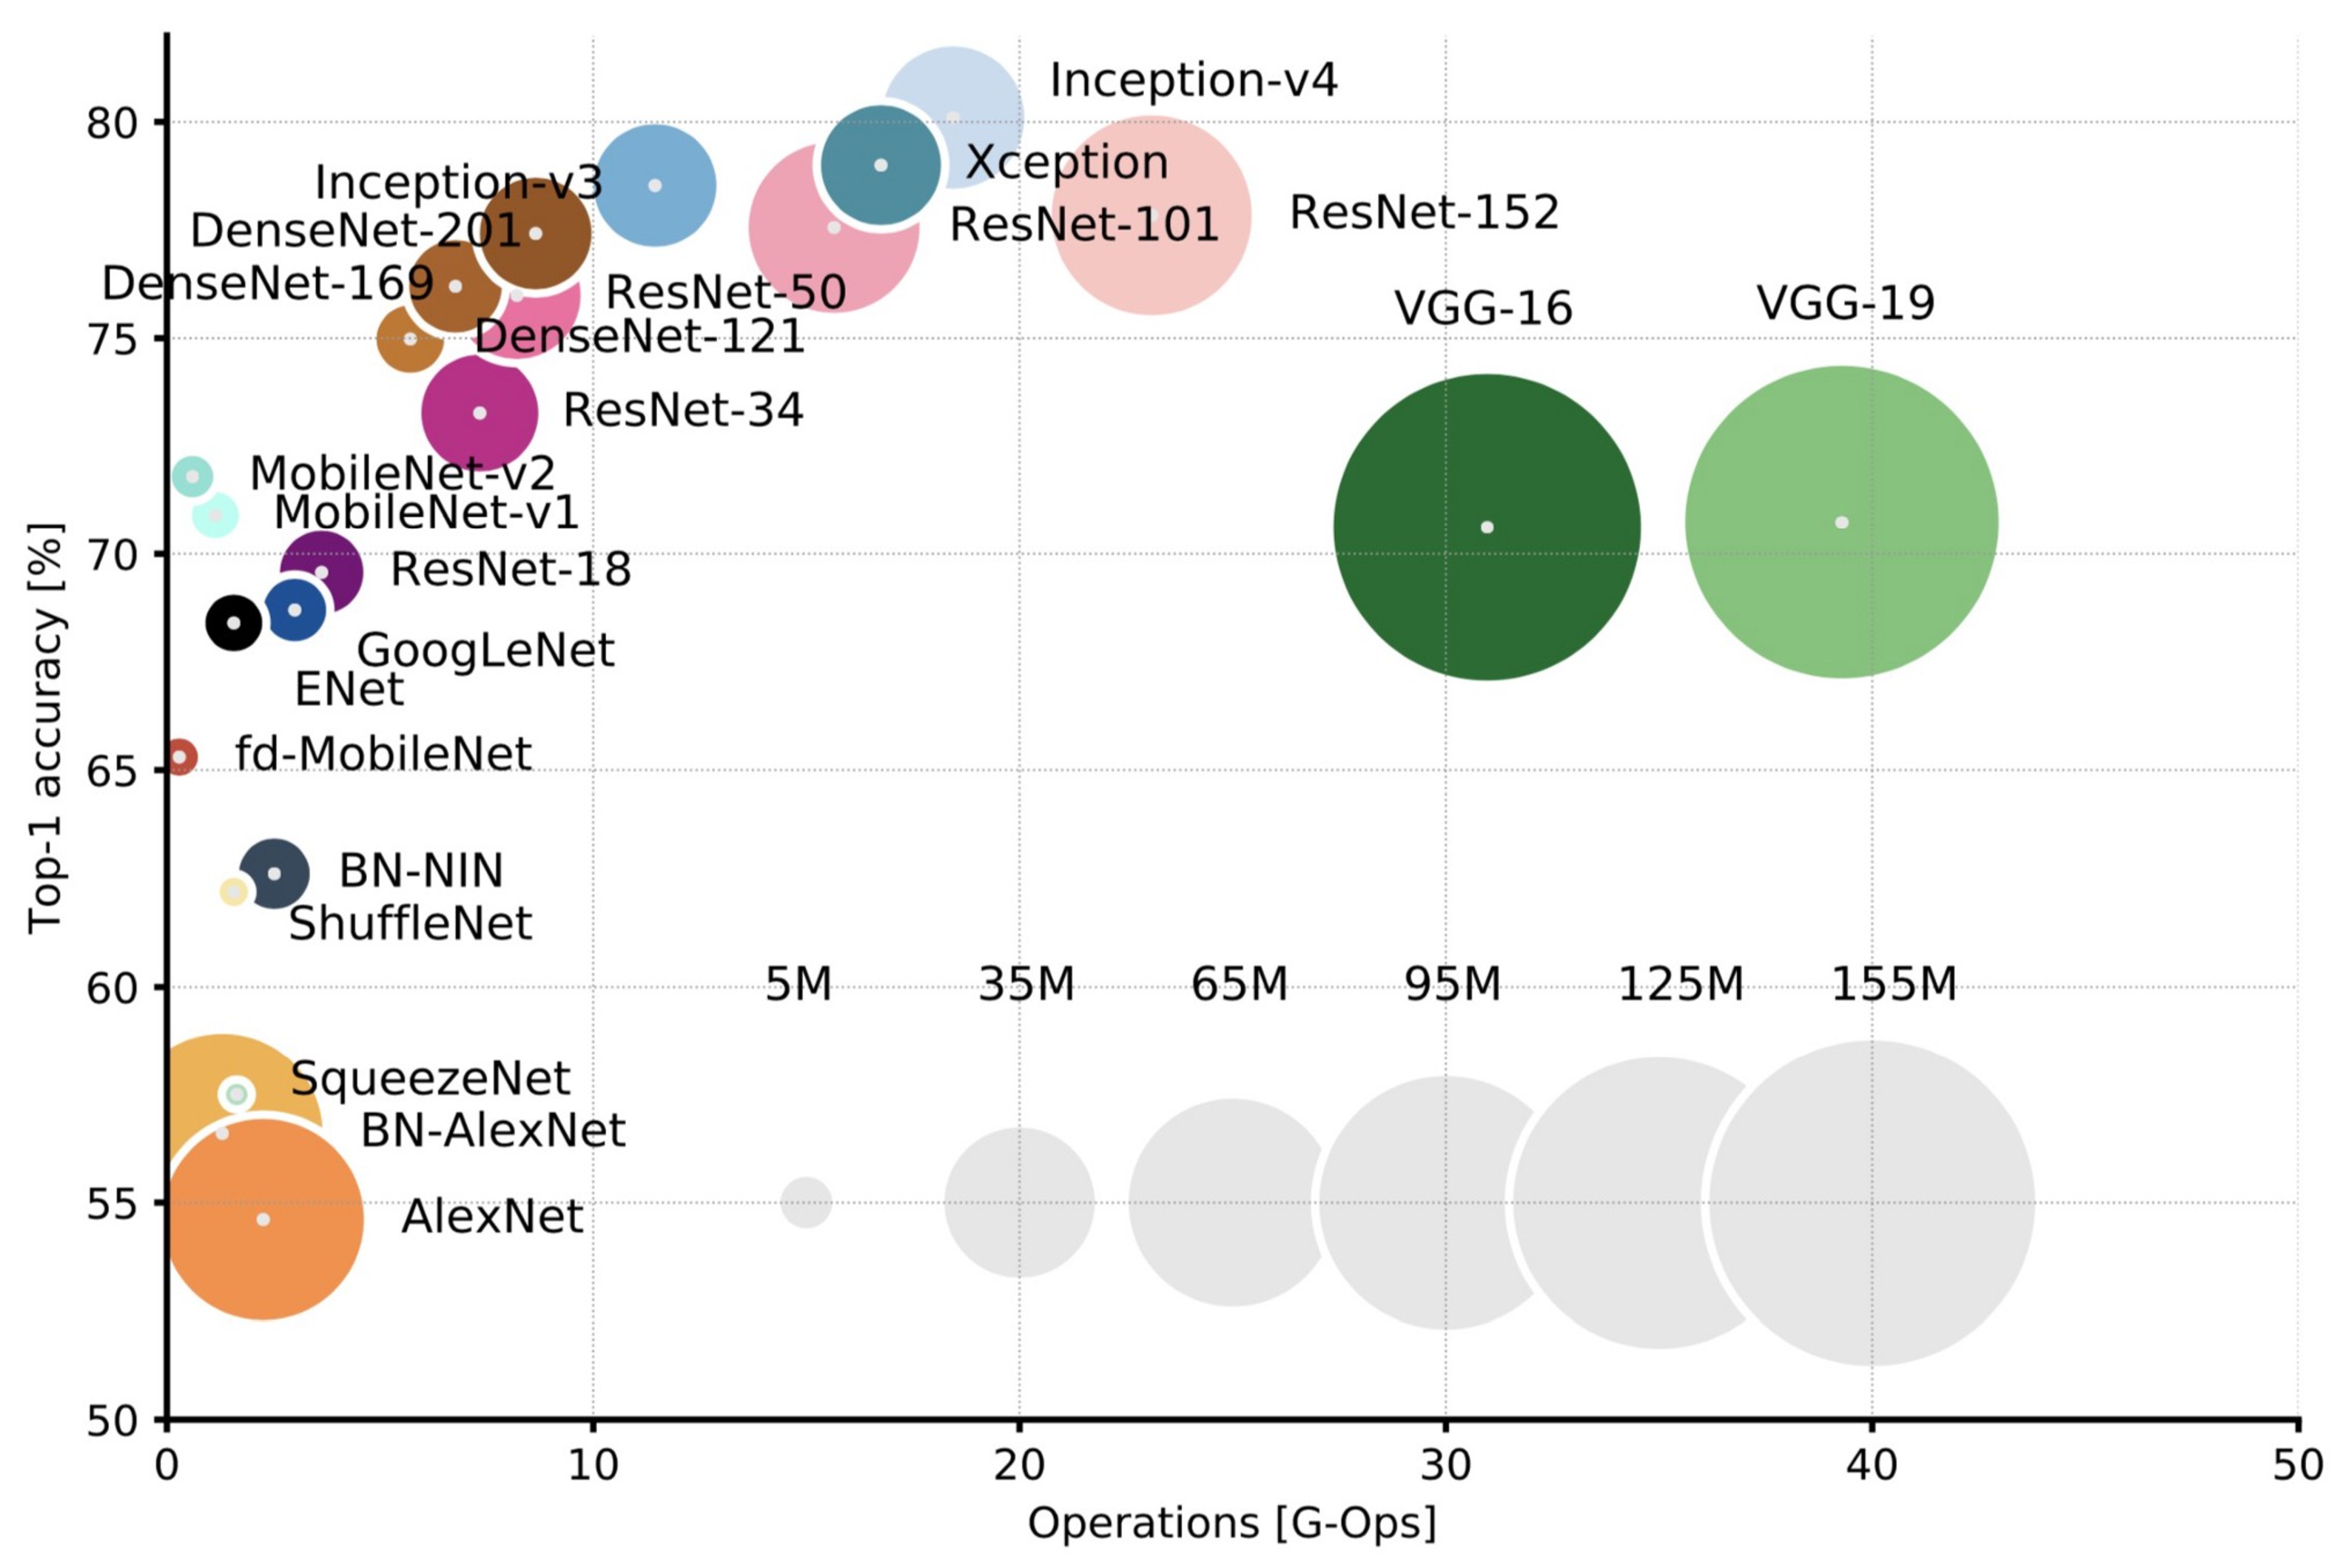
\includegraphics[width=0.9\textwidth]{archi.pdf}
    \caption{Ball chart reporting the Top-1 accuracy of various architectures vs. their computational complexity \cite{canziani_analysis_2017}}
    \label{fig:archi}
\end{figure}
%
\subsubsection{Pruning} \label{subs:pruning}
%
To improve the inference phase of a \acrshort{cnn}, pruning can be used, especially for applications with limited computational resources \cite{liu_rethinking_2019}. According to \textcite{liu_rethinking_2019, denton_exploiting_2014}, the huge number of parameters in a network might create a problem of \textbf{over-parametrization}. Over-parametrization means that there are redundancies in \acrshort{nn} parameters and that the same performance could be achieved with only a subset of them. In other words, a lot of parameters are unimportant or unnecessary \cite{cheng_recent_2018}. Pruning is defined as removing the parameters considered as not important. For example, \textcite{baoyuan_liu_sparse_2015} achieve more than 90\% sparsity of parameters in convolutional layers in AlexNet with less than 1\% accuracy loss.

We can explain why pruning works by \textbf{The Lottery Ticket Hypothesis} \cite{frankle_lottery_2018, frankle_early_2020}: \textquote{\textit{A randomly-initialized, dense neural network contains a subnetwork that is initialized such that—when trained in isolation—it can match the test accuracy of the original network after training for at most the same number of iterations.}} From this postulate, those unimportant weights can be set to zero (prune) because they do not improve the accuracy of the model.

According to \textcite{cheng_recent_2018}, pruning has two major benefits for the inference phase. First, less storage is required. Indeed, the non-pruned weights are sparsely distributed among the kernels. Thus, they can be stored in a compressed format reducing memory utilization. Second, pruning reduces the arithmetic complexity of the network. As convolutions perform a weighted sum with the input \acrshort{fm}, each \acrfull{mac} operation with a pruned weight can be discarded. Moreover, \textcite{han_learning_2015, mao_exploring_2017, kang_accelerator-aware_2020} pointed out that some pruning ratios can also improve the accuracy of the network, which can be explained by a form of regularization.

Various pruning schemes are focused on increasing the sparsity of the network without a drop of accuracy \cite{han_deep_2016, han_learning_2015}.  We call this pruning scheme where all unimportant parameters are pruned without extra constraint \textbf{unstructured pruning} \cite{cheng_recent_2018}. However, it is challenging to exploit the performance and the high parallelism of \acrshort{fpga} with this kind of pruned network. Indeed, this kind of pruning scheme creates irregularities in the data access pattern \cite{zhu_efficient_2020}. It means that the number of pruned weights is different in each kernel, and we should adapt the circuitry to the worst case. As a consequence, all filters conduct wasteful operations except the worst case \cite{shimoda_filter-wise_2019}. Furthermore, \textcite{anwar_structured_2017} pointed out that unstructured pruning requires overhead for computing addresses of the sparse non-pruned elements. Therefore, we should find pruning patterns that would be more hardware-friendly.

In contrast to the unstructured pruning, we have \textbf{structured pruning} schemes \cite{kang_accelerator-aware_2020}. They combine a structure regularization for accuracy and locality optimization for computation efficiency. According to \textcite{anwar_structured_2017}, \textquote{\textit{Structured pruning has no or little extra costs}}. We can categorize the various schemes into different groups \cite{cheng_recent_2018, kang_accelerator-aware_2020, anwar_structured_2017, wen_learning_2016}:
\begin{itemize}
    \item \textbf{Depth-wise}: all the weights of a layer are pruned. The layer is then removed.
    \item \textbf{Kernel-wise}: instead of pruning all the weights, we keep a ratio of kernels, which means a reduction of the number of outputs channel. This pruning scheme is provided in Figure \ref{fig:struct_pruning:fw}.
    \item \textbf{Channel-wise}: it is one of the most popular methods because it still can fit in the convolutional deep learning frameworks \cite{liu_rethinking_2019}. A layer of the input \acrshort{fm} is pruned, which means that the layer is also pruned in all the kernels, as can be seen in Figure \ref{fig:struct_pruning:chw}.
    \item \textbf{Shape-wise}: we prune the same weight in each kernel or group of kernels. For example, this pruning scheme has been used in \textcite{zhu_efficient_2020}. It is illustrated in Figure \ref{fig:struct_pruning:sw}
\end{itemize}
%
\begin{figure}[H]
    \centering
    %
    \begin{subfigure}[t]{.32\textwidth}
    \centering
    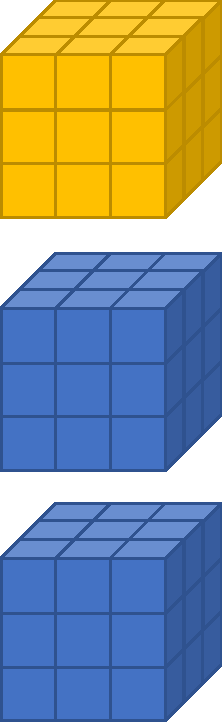
\includegraphics[width=0.33\linewidth]{filterwise.pdf}
    \caption{kernel-wise pruning}
    \label{fig:struct_pruning:fw}
    \end{subfigure}
    %
    \begin{subfigure}[t]{.32\textwidth}
    \centering
    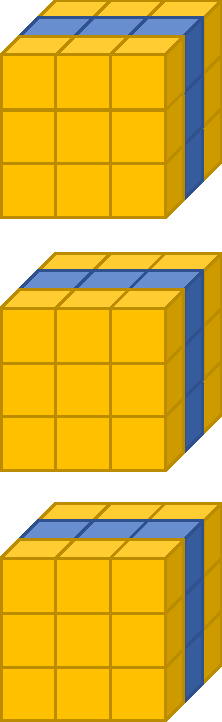
\includegraphics[width=0.33\linewidth]{channelwise.pdf}
    \caption{channel-wise pruning}
    \label{fig:struct_pruning:chw}
    \end{subfigure}
    %
    \begin{subfigure}[t]{.32\textwidth}
    \centering
    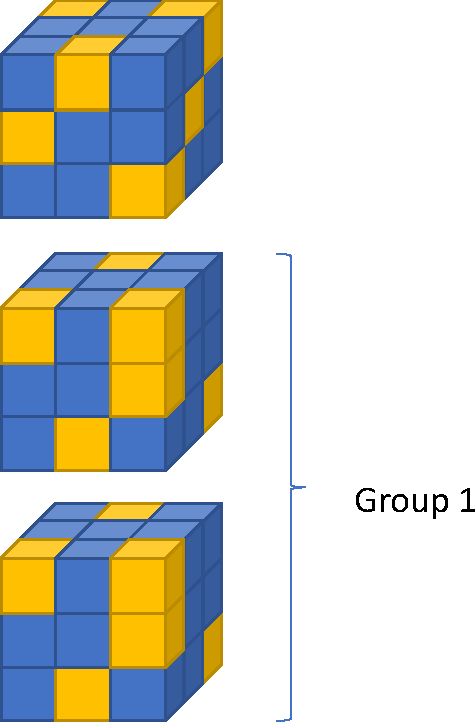
\includegraphics[width=0.70\linewidth]{shapewise.pdf}
    \caption{shape-wise pruning}
    \label{fig:struct_pruning:sw}
    \end{subfigure}
    %
    \caption{Structured pruning schemes, where the yellow weights are the pruned ones, inspired by \cite{cheng_recent_2018}}
    \label{fig:struct_pruning}
\end{figure}
%
The previously cited pruning schemes are ordered from very coarse-grained to fine-grained sparsity \cite{mao_exploring_2017}. As explained previously, coarse-grained sparsity (channel-wise and filter-wise pruning) provides a higher acceleration and can be used when implementing \acrshort{cnn} on \acrshort{gpu} or \acrshort{cpu} \cite{cheng_recent_2018, mao_exploring_2017}. However, finer-grained ones provide higher accuracy and as the sparsity increases, the accuracy is less affected, as can be seen in Figure \ref{fig:pruning-accuracy}. Therefore, this work focuses on developing customized hardware that can exploit a more fine-grained sparsity \cite{mao_exploring_2017} to provide a higher pruning while limiting the drop of accuracy.
%
\begin{figure}[H]
    \centering
    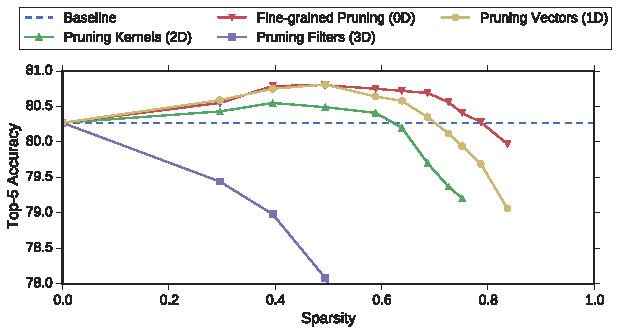
\includegraphics[width=\textwidth]{accuracysparsity.pdf}
    \caption{Accuracy-Sparsity Curve of AlexNet obtained by pruning \cite{mao_exploring_2017}}
    \label{fig:pruning-accuracy}
\end{figure}
%
Some studies focused on the acceleration of the inference step of lightweight models thanks to pruning. \textcite{zhang_channel_2019, tu_pruning_2019} applied pruning on \acrshort{dsc} kernels. They both chose \textbf{Channel-wise} pruning because it does not create sparse connections and it efficiently improves the speed of the inference. It also reduces the computational cost of the $1 \times 1$ (pointwise) convolutions, where the majority of the parameters and the \acrshort{mac} come from. In MobileNet, it is about 95\%. By discarding one channel, the associated depthwise convolution is also avoided.
Moreover, the pointwise kernel producing that channel in the previous block can also be pruned. We can see the process in Figure \ref{fig:pruning_dsc}.
%
\begin{figure}[H]
    \centering
    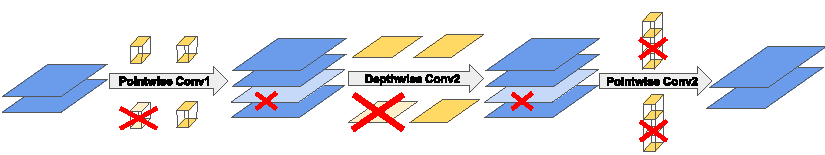
\includegraphics[width=\textwidth]{channelwise_ex.pdf}
    \caption{Pruning a depthwise separable convolution \cite{tu_pruning_2019}}
    \label{fig:pruning_dsc}
\end{figure}

\textbf{In this work, we focus on a structured pruning scheme for depthwise separable convolution. More precisely, we develop an architecture on \acrshort{fpga} than combines both advantages of pruning and depthwise separable convolution.}
%
\subsubsection{Quantization} \label{subs:quantization}
%
%
Quantization is an approach to trade accuracy for a decrease of the storage requirements of a network \cite{han_deep_2016}. Indeed, we can define quantization as the reduction of the number of bits representing a weight or pixel. Moreover, instead of using a floating-point number, we can use a \textbf{fixed-point number} \cite{cheng_recent_2018}. As said previously, fixed-point numbers are known to be more efficient on hardware such as \acrshort{fpga} because we can use integer arithmetic \cite{david_hardware_2007}. Quantization to fixed-point numbers can then reduce the memory requirement and the latency of the inference stage.

The format to encode the fixed-point representation of a real number is the \textit{Q-format} \cite{ward_real-time_2001}. A N-bit number, noted $Q_{m.n}$, is divided into two parts separated by an implied binary point. The $m$ bits are used to represent the integer part of the number (including the sign bit), and the $n$ bits are used to represent the fractional part, as can be seen in Figure \ref{fig:Qformat}. The bitwidth associated with each part can be either the same, either fine-tuned for each layer after analysis. Indeed, \textcite{qiu_going_2016, yin_high_2018} choose a different range for each layer, but doing it for every weight is not memory-efficient.
%
\begin{figure}[H]
    \centering
    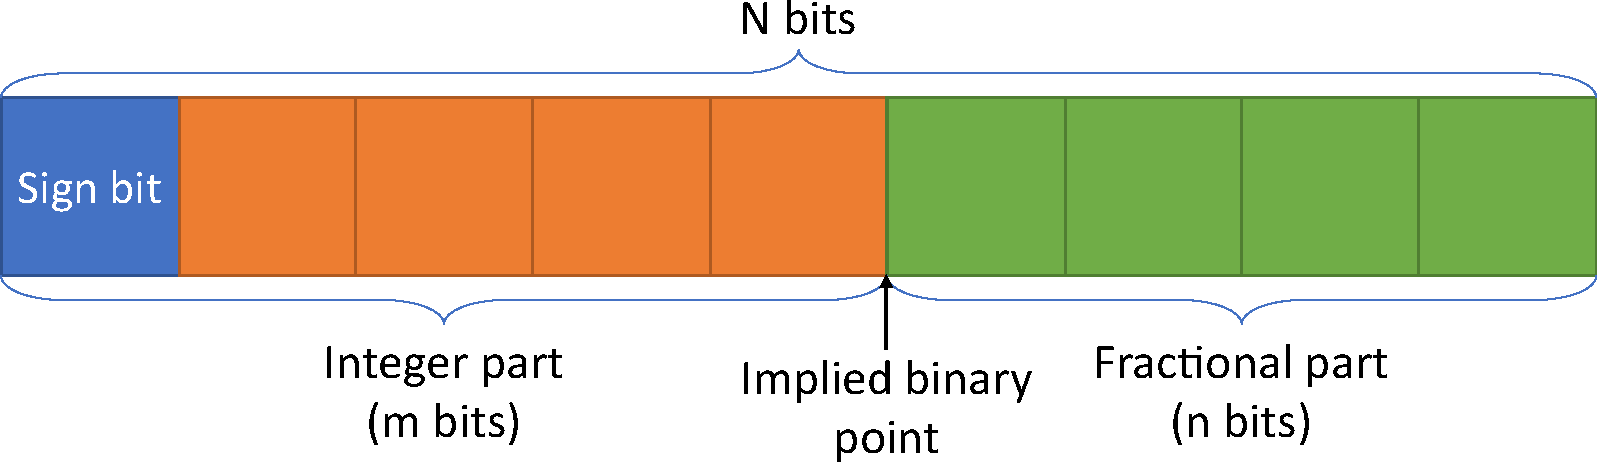
\includegraphics[width=\textwidth]{Qformat.pdf}
    \caption{Illustration of the Q-format}
    \label{fig:Qformat}
\end{figure}

As pointed out by \textcite{han_deep_2016}, quantization and pruning techniques are orthogonal and can be combined to compress further the network. Unfortunately, not all existing networks are friendly for quantization, like MobileNet. MobiletNet with quantized pixels and weights has a large drop of accuracy compared with its Non-quantized version (70.50\% using floating-point model vs 1.80\% using an 8-bit pipeline) \cite{sheng_quantization-friendly_2018}. However, the work of \textcite{sheng_quantization-friendly_2018} showed that the source of the accuracy drop was the design of the separable convolution core layer. They proposed therefore a new quantization-friendly separable convolution core layer. Works on MobileNetV2 should then be done to verify the fixed-point inference accuracy. Still, an 8-bit pipeline might not be optimal for MobilNet as increasing the bitwidth to 16-bit could boost accuracy \cite{cheng_recent_2018}. This bitwidth is also widely used \cite{huimin_li_high_2016, bai_cnn_2018}. 

\textbf{Therefore, 16-bit fixed-point Q-format is adopted for input data, weights, and intermediate data in the frame of this thesis}. \textbf{Moreover, as said previously in Section \ref{subs:acti}, we can limit the integer part to 3 bits (one bit is added to express the sign of the weights), and we can use $Q_{4.12}$.}
